\documentclass[fleqn, a4paper, 11pt, oneside]{amsart}
%\usepackage[top = 2cm, bottom = 1cm, left = 1cm, right = 1cm]{geometry}
\usepackage{exsheets, tasks}
\usepackage{amsmath, amssymb, amsthm} %standard AMS packages
\usepackage{marginnote} %marginnotes
\usepackage{gensymb} %miscellaneous symbols
\usepackage{commath} %differential symbols
\usepackage{xcolor} %colours
\usepackage{cancel} %cancelling terms
\usepackage{siunitx} %formatting units
\usepackage{tikz, pgfplots} %diagrams
\usetikzlibrary{calc, hobby, patterns, intersections}
\usepackage{graphicx} %inserting graphics
\usepackage{hyperref} %hyperlinks
\usepackage{datetime} %date and time
\usepackage{ulem} %underline for \emph{}
\usepackage{xfrac} %inline fractions
\usepackage{enumerate,enumitem} %numbered lists
\usepackage{float} %inserting floats
\usepackage{circuitikz} %circuit diagrams

\newcommand\numberthis{\addtocounter{equation}{1}\tag{\theequation}} %adds numbers to specific equations in non-numbered list of equations

\newcommand{\AxisRotator}[1][rotate=0]{
	\tikz [x=0.25cm,y=0.60cm,line width=.2ex,-stealth,#1] \draw (0,0) arc (-150:150:1 and 1);%
} %rotation symbols on axes

\theoremstyle{definition}
\newtheorem{example}{Example}
\newtheorem{definition}{Definition}

\theoremstyle{theorem}
\newtheorem{theorem}{Theorem}

\newcommand{\curl}{\mathrm{curl\,}}

\makeatletter
\@addtoreset{section}{part} %resets section numbers in new part
\makeatother

\renewcommand{\thesubsection}{(\arabic{subsection})}
\renewcommand{\thesection}{(\arabic{section})}

%section headings on left
\makeatletter
\def\specialsection{\@startsection{section}{1}%
	\z@{\linespacing\@plus\linespacing}{.5\linespacing}%
	%  {\normalfont\centering}}% DELETED
	{\normalfont}}% NEW
\def\section{\@startsection{section}{1}%
	\z@{.7\linespacing\@plus\linespacing}{.5\linespacing}%
	%  {\normalfont\scshape\centering}}% DELETED
	{\normalfont\scshape}}% NEW
\makeatother

%forces newline after subsection
\makeatletter
\def\subsection{\@startsection{subsection}{3}%
	\z@{.5\linespacing\@plus.7\linespacing}{.1\linespacing}%
	{\normalfont\itshape}}
\makeatother

\settasks{counter-format = tsk[1].}

\SetupExSheets{solution/print = true}

%opening
\title{Physics 2 : Assignment 6}
\author
{
	Aakash Jog\\
	ID : 989323563
}
\date{\formatdate{6}{5}{2015}}

\begin{document}

\maketitle
%\setlength{\mathindent}{0pt}

\begin{question}
	A sphere of linear dielectric material has embedded in it a uniform free charge density $\rho$.
	Find the potential at the center of the sphere (relative to infinity), if its radius $R$ and its dielectric constant is $\varepsilon_r$.
\end{question}

\begin{solution}
	Consider a spherical Gaussian surface just outside the surface of the sphere.\\
	By Gauss' Law in dielectrics,
	\begin{align*}
		\int \varepsilon_r E \dif A &= Q\\
		\therefore \varepsilon_r E \cdot 4 \pi R^2 &= \rho \cdot \frac{4}{3} \pi R^3\\
		\therefore E &= \frac{\rho R}{3 \varepsilon_r}
	\end{align*}
	Outside the sphere,
	\begin{align*}
		E &= \frac{1}{4 \pi \varepsilon_0} \frac{\frac{4}{3} \pi R^3 \rho}{r^2}\\
		&= \frac{\rho R^3}{3 \varepsilon_0 r^2}
	\end{align*}
	Therefore,
	\begin{align*}
		\varphi_{\textnormal{centre}} &= -\int\limits_{\infty}^{0} E \cdot \dif r\\
		&= -\int\limits_{\infty}^{R} \frac{\rho R^2}{3 \varepsilon_0 r^2} \dif r - \int\limits_{R}^{0} \frac{\rho R}{3 \varepsilon_r} \dif r\\
		&= \frac{\rho R^2}{3 \varepsilon_0} \left( 1 + \frac{1}{2 \varepsilon_r} \right)
	\end{align*}
\end{solution}

\begin{question}
	A certain coaxial cable consists of a copper wire, radius $a$, surrounded by a concentric copper tube of inner radius $b$ and outer radius $c$, as shown.
	The space between is partially filled (from $b$ to $c$), with material of dielectric constant $\varepsilon_r$, as shown.
	Find the capacitance per unit length of this cable.
	\begin{figure}[H]
		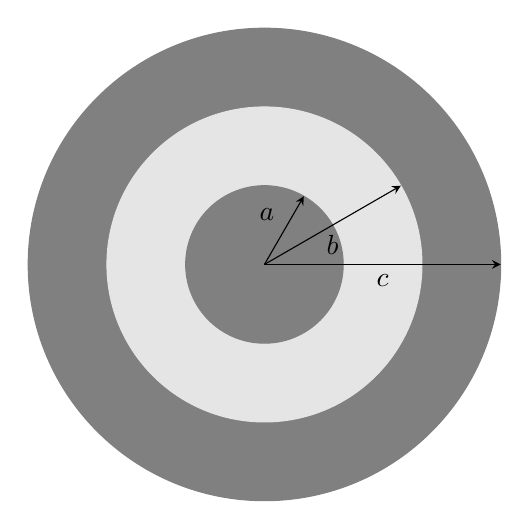
\begin{tikzpicture}
			\def\a{1};
			\def\b{2};
			\def\c{3};

			\filldraw [gray] (0,0) circle (\c);
			\filldraw [white!90!black] (0,0) circle (\b);
			\filldraw [gray] (0,0) circle (\a);

			\begin{scope}[-stealth]
				\draw (0,0) -- (0:\c) node [midway, below] {$c$};
				\draw (0,0) -- (30:\b) node [midway, below] {$b$};
				\draw (0,0) -- (60:\a) node [midway, above left] {$a$};
			\end{scope}
		\end{tikzpicture}
	\end{figure}
\end{question}

\begin{solution}
	Let the charge on the surfaces of radii $a$ and $b$ be $Q$ and $-Q$ respectively.\\
	Consider a cylindrical Gaussian surface with radius $r$ and length $l$.\\
	Therefore, by Gauss' Law,\\
	If $a < r < b$,
	\begin{align*}
		E &= \frac{Q}{2 \pi \varepsilon_0 r l}
	\end{align*}
	If $b < r < c$,
	\begin{align*}
		E &= \frac{Q}{2 \pi \varepsilon_r r l}
	\end{align*}
	Therefore,
	\begin{align*}
		V &= -\int\limits_{c}^{a} E \dif r\\
		&= -\int\limits_{c}^{b} \frac{Q}{2 \pi \varepsilon_r r l} \dif r - \int\limits_{b}^{a} \frac{Q}{2 \pi \varepsilon_0 r l} \dif r\\
		&= \frac{Q}{2 \pi l} \left( \frac{1}{\varepsilon_0} \ln \left( \frac{b}{a} \right) + \frac{1}{\varepsilon_r} \ln \left( \frac{c}{b} \right) \right)
	\end{align*}
	Therefore,
	\begin{align*}
		C &= \frac{Q}{V}\\
		\therefore \frac{C}{l} &= \frac{Q}{V l}\\
		&= \frac{2 \pi }{\frac{1}{\varepsilon_0} \ln \left( \frac{b}{a} \right) + \frac{1}{\varepsilon_r} \ln \left( \frac{b}{a} \right)}
	\end{align*}
\end{solution}

\begin{question}
	Calculate the attraction force between the plates of a capacitor carrying charge $q$.
	Using this result show that the force per unit area acting on either plate is given by $\frac{1}{2} \varepsilon_0 E^2$.
	Note: this result is true for a conductor of any shape with electric field $\overrightarrow{E}$ at its surface.
\end{question}

\begin{solution}
	Let the area of the capacitor plates be $A$, the charge of each of them be $\pm Q$, and the distance between them be $l$.\\
	Therefore,
	\begin{align*}
		U &= \frac{Q^2}{2 C}\\
		&= \frac{Q^2}{2 A \frac{\varepsilon_0}{l}}\\
		&= \frac{Q^2 l}{2 A \varepsilon_0}
	\end{align*}
	Therefore,
	\begin{align*}
		F &= \dod{U}{l}\\
		&= \frac{Q^2}{2 A \varepsilon_0}
	\end{align*}
	Therefore,
	\begin{align*}
		\frac{F}{A} &= \frac{Q^2}{2 A^2 \varepsilon_0}\\
		&= \frac{\sigma^2}{2 \varepsilon_0}\\
		&= \frac{1}{2} \left( \frac{\sigma}{\varepsilon_0} \right)^2 \varepsilon_0\\
		&= \frac{1}{2} \varepsilon_0 E^2
	\end{align*}
\end{solution}

\begin{question}
	A dielectric slab of thickness $b$ is inserted between the plates of a parallel-plate capacitor of plate separation $d$.
	Calculate the capacitance.
\end{question}

\begin{solution}
	Let the permittivity of the dielectric material be $\varepsilon$.\\
	Let the distances between the plates and the edges of the slab be as shown.
	\begin{figure}[H]
		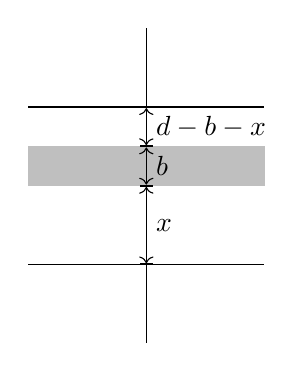
\begin{tikzpicture}
			\def\a{3};
			\def\b{0.5};
			\def\d{2};
			\def\x{1};

			\begin{scope}
				\draw (-\a/2,0) -- (\a/2,0);
				\draw (-\a/2,\d) -- (\a/2,\d);

				\draw (0,0) -- ++(0,-\d/2);
				\draw (0,\d) -- ++(0,\d/2);
			\end{scope}

			\begin{scope}
				\filldraw [lightgray] (-\a/2,\x) rectangle (\a/2, \x + \b);
			\end{scope}

			\begin{scope}[|<->|]
				\draw (0,0) -- (0,\x) node [midway, right] {$x$};
				\draw (0,\x) -- (0,\x + \b) node [midway, right] {$b$};
				\draw (0,\x + \b) -- (0,\d) node [midway, right] {$d - b - x$};
			\end{scope}
		\end{tikzpicture}
	\end{figure}
	Therefore, the arrangement is equivalent to three capacitors in series.\\
	Let the capacitances of the three be $C_1$, $C_2$, $C_3$, respectively.\\
	Therefore,
	\begin{align*}
		\frac{1}{C} &= \frac{1}{C_1} + \frac{1}{C_2} + \frac{1}{C_3}\\
		&= \frac{d - b - x}{A \varepsilon_0} + \frac{b}{A \varepsilon} + \frac{x}{A \varepsilon_0}\\
		&= \frac{d - b}{A \varepsilon_0} + \frac{b}{A \varepsilon}\\
		\therefore C &= -\frac{A \varepsilon \varepsilon_0}{\varepsilon (b - d) - b \varepsilon_0}
	\end{align*}
\end{solution}

\begin{question}
	Find the equivalent capacitance between points $x$ and $y$ in
	\begin{figure}[H]
		\begin{circuitikz}[scale = 1.5]
			\draw
				(0,0) to (1,0)
				(1,0) to [C = $C_1$] (2,0)
				(2,0) to [C = $C_2$] (3,0)
				(3,0) to [C = $C_3$] (4,0)
				(4,0) to (5,0);
			\draw
				(1,0) to (1,1)
				(1,1) to [C = $C_4$] (3,1)
				(3,1) to (3,0);
			\draw
				(2,0) to (2,-1)
				(2,-1) to [C = $C_5$] (4,-1)
				(4,-1) to (4,0);
			\foreach \i in {0,...,5}
			{
				\filldraw (\i,0) circle (1pt);
			}
			\node [left] at (0,0) {$x$};
			\node [right] at (5,0) {$y$};
		\end{circuitikz}
	\end{figure}
	Assume that $C_2 = 10 \si{\micro\farad}$ and that the other capacitors are all $4 \si{\micro\farad}$.
\end{question}

\begin{solution}
	As all of $C_1$, $C_3$, $C_4$, $C_5$ are equal, the Wheatstone bridge is balanced.\\
	Therefore the current through it is zero.\\
	Hence, the circuit is equivalent to
	\begin{figure}[H]
		\begin{circuitikz}[scale = 1.5]
			\draw
				(0,0) to (1,0)
				(1,0) to [C = $C_1$] (2,0)
				(3,0) to [C = $C_3$] (4,0)
				(4,0) to (5,0);
			\draw
				(1,0) to (1,1)
				(1,1) to [C = $C_4$] (3,1)
				(3,1) to (3,0);
			\draw
				(2,0) to (2,-1)
				(2,-1) to [C = $C_5$] (4,-1)
				(4,-1) to (4,0);
			\foreach \i in {0,...,5}
			{
				\filldraw (\i,0) circle (1pt);
			}
			\node [left] at (0,0) {$x$};
			\node [right] at (5,0) {$y$};
		\end{circuitikz}
	\end{figure}
	Therefore,
	\begin{align*}
		C &= \frac{C_1 C_5}{C_1 + C_5} + \frac{C_3 C_4}{C_3 + C_4}\\
		&= \frac{16}{8} + \frac{16}{8}\\
		&= 4 \si{\micro\farad}
	\end{align*}
\end{solution}

\end{document}
